\documentclass[10pt,a4paper,titlepage]{report}
\usepackage[utf8]{inputenc}
\usepackage{amsmath}
\usepackage{amsfonts}
\usepackage{amssymb}
\usepackage{graphicx}
\usepackage{xcolor}
\usepackage{minted}
\nonstopmode


\begin{document}
\begin{titlepage}
\author{Rwithik Manoj}
\title{Shell Scripting\\Set 2\\Part b}
\date{\today}
\maketitle
\end{titlepage}

\begin{enumerate}
\item Write a shell script that will take an input file and remove identical lines. \newline
\textbf{Algorithm}:\newline
\begin{enumerate}
	\item Start.
	\item Exit the script if the file does not exist.
	\item Use {\color{red}awk `!seen[\$0]++' } to remove duplicate lines.
	\item This makes a dictionary, named seen. When a new line is encountered, it sets the value of the key as one. It prints the lie only if the value of seen[\$0] is zero. So the next time the same line is encountered, it is not printed.
	\item Stop.
\end{enumerate}
\newline
\textbf{Script:}\newline
\inputminted{bash}{../Scripts/Set2/6.sh}
\textbf{Output:}\newline
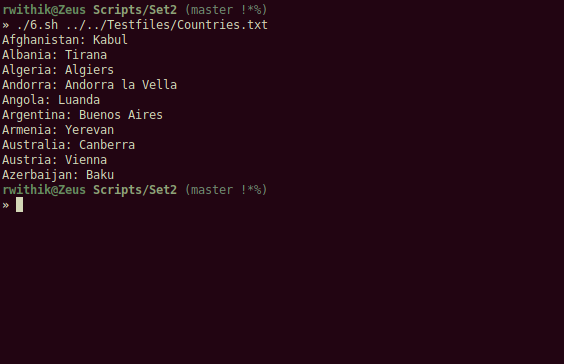
\includegraphics[width=\linewidth]{../Images/Shell2/6.png}
\pagebreak
\item Write a shell script that displays a list of all the files in the current directory to which the user has read, write and execute permissions. \newline
\textbf{Algorithm}:\newline
\begin{enumerate}
	\item Start.
	\item Write the contents of the current directory to a file, f.
	\item Redirect the input stream to the file.
	\item Check the permissions of the file with the {\color{red}-r}, {\color{red}-w} and {\color{red}-x} flags of {\color{red}test}.
	\item Stop.
\end{enumerate}
\newline
\textbf{Script:}\newline
\inputminted{bash}{../Scripts/Set2/7.sh}
\newline
\textbf{Output:}\newline
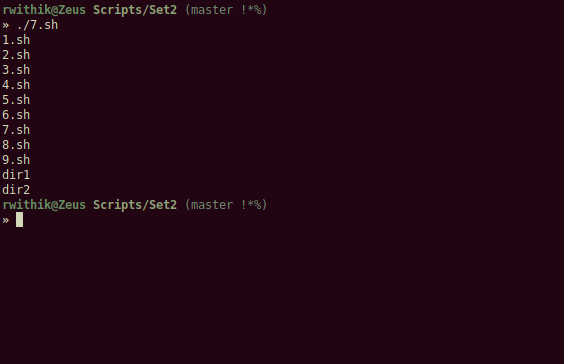
\includegraphics[width=\linewidth]{../Images/Shell2/7.png}
\pagebreak

\item Write a shell script that folds long lines into 40 columns. Thus any line that exceeds 40 characters must be broken after 40th. A \textbackslash  is to be appended as the indication of folding and the processing is to be continued with the residue. The input is to be through a text file created by the user. \newline
\textbf{Algorithm}:\newline
\begin{enumerate}
	\item Start.
	\item Exit the script if the file doesn't exist.
	\item Store the number of lines in a variable, n.
	\item Iterate through the file.
	\item Loop through the line and cut 40 characters in each iteration.
	\item Stop.
\end{enumerate}
\newline
\textbf{Script:}\newline
\inputminted{bash}{../Scripts/Set2/8.sh}
\newline
\textbf{Output:}\newline
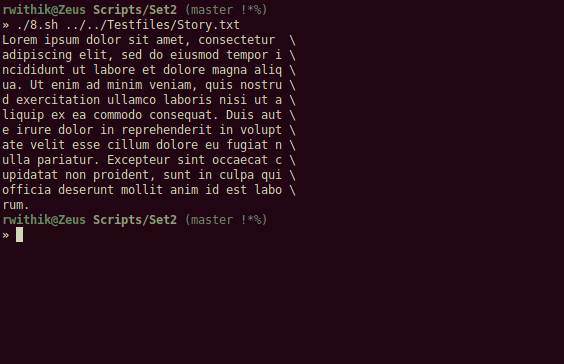
\includegraphics[width=\linewidth]{../Images/Shell2/8.png}
\pagebreak

\item Write a shell script to delete all lines containing a specific word in one or more file supplied as argument to it. \newline
\textbf{Algorithm}:\newline
\begin{enumerate}
	\item Start.
	\item Read the word.
	\item Loop through the files.
	\item Check of the file exists.
	\item Delete the lines contaning the word, with {\color{red}sed}.
	\item Stop.
\end{enumerate}
\newline
\textbf{Script:}\newline
\inputminted{bash}{../Scripts/Set2/9.sh}
\newline
\textbf{Output:}\newline
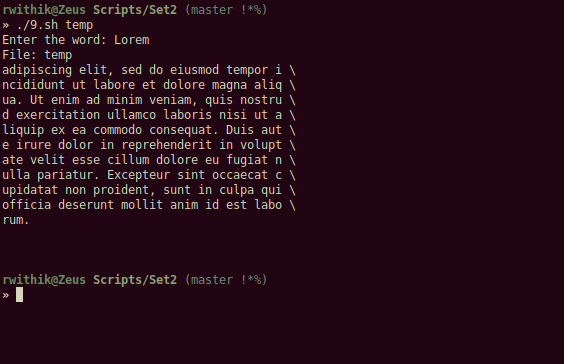
\includegraphics[width=\linewidth]{../Images/Shell2/9.png}
\end{enumerate}

\end{document} 
